	\documentclass[10pt,oneside]{CBFT_book}
	% Algunos paquetes
	\usepackage{amssymb}
	\usepackage{amsmath}
	\usepackage{graphicx}
	\usepackage{libertine}
	\usepackage[bold-style=TeX]{unicode-math}
	\usepackage{lipsum}

	\usepackage{natbib}
	\setcitestyle{square}

	\usepackage{polyglossia}
	\setdefaultlanguage{spanish}
	



	\usepackage{CBFT.estilo} % Cargo la hoja de estilo

	% Tipografías
	% \setromanfont[Mapping=tex-text]{Linux Libertine O}
	% \setsansfont[Mapping=tex-text]{DejaVu Sans}
	% \setmonofont[Mapping=tex-text]{DejaVu Sans Mono}

	%===================================================================
	%	DOCUMENTO PROPIAMENTE DICHO
	%===================================================================

\begin{document}

% =================================================================================================
\chapter{Métodos perturbativos}
% =================================================================================================

Se basan en 
\[
	H = H_0 + \lambda V \qquad \lambda \ll 1 \; \text{$\lambda$ es un parámetro para controlar
	la perturbación}
\]
con $ H_0\Ket{n^{(0)}} = E_n^{(0)}\Ket{n^{(0)}}$ (el problema sin perturbar)
\[
	H \Ket{n(\lambda)} = E_n(\lambda) \Ket{n(\lambda)}
\]
que sería la solución exacta.
Como esto es hartocomplicado podemos desarrollar en serie 
\[
	E_n(\lambda) \approx E_n^0 + \lambda E_n^1 + \lambda^2 E_n^2 
\]
\[
	\Ket{n(\lambda)} \approx \Ket{0_n} + \lambda \Ket{1_n} + \lambda^2  \Ket{2_n}
\]
siendo $n$ autoestado correspondiente y $(0),(1),(2)$ los órdenes del desarrollo perturbativo.
Luego,
\[
	\left( H_0 + \lambda V \right)\left[ \sum_{i=0}^{\infty} \lambda^i\Ket{i_n} \right] =
	\left(\sum_{j=0}^{\infty} \lambda^j E_n^{(j)}\right)\left(\sum_{i=0}^{\infty} \lambda^i\Ket{i_n}\right)
\]
\[
	\sum_{i=0}^\infty H_0 \lambda^i \Ket{i_n} + \lambda V \lambda^i \Ket{i_n} =
	\sum_{i,j} \lambda^j E_n^j \lambda^i \Ket{i_n}
\]
y aproximando los primeros términos 
\[
	H_0\Ket{0_n} + H_0\lambda\Ket{1_n} + H_0\lambda^2\Ket{2_n} + V\lambda\Ket{0_n} +
	V\lambda^2\Ket{1_n}+... =
\]
\[
	E_n^0\Ket{0_n} + E_n^0\lambda\Ket{1_n} + E_n^0\lambda^2\Ket{2_n} +
	E_n^1\lambda\Ket{0_n} + E_n^1\lambda^2\Ket{1_n} + E_n^1\lambda^3\Ket{2_n} + 
	E_n^2\lambda^2\Ket{0_n}
\]
ahora igualamos orden a orden y resulta 
\[
	\lambda^0 .... H_0\Ket{0_n}  = E_n^0\Ket{0_n}
\]
\[
	\lambda^1 .... H_0\Ket{1_n} + V\Ket{0_n} = 
	E_n^0\Ket{1_n} + E_n^1\Ket{0_n} 
\]
\[
	\lambda^2 .... H_0\Ket{2_n} + V\Ket{1_n} =
	E_n^0\Ket{2_n} + E_n^2\Ket{0_n} + E_n^1\Ket{1_n}
\]

Pediremos una normalización a cada orden y considerando $ \Braket{0_n|n(\lambda)} \in \mathbb{R}$
\[
	\left( \Bra{0_n} + \lambda\Bra{1_n} + \lambda^2\Bra{2_n} \right)
	\left( \Ket{0_n} + \lambda\Ket{1_n} + \lambda^2\Ket{2_n} \right) =
\]
\[
\begin{aligned}
 \Braket{0_n|0_n} +& \lambda\Braket{1_n|0_n} +& \lambda^2 \Braket{2_n|0_n} &  & & \\
 & \lambda\Braket{0_n|1_n} +& \lambda^2\Braket{1_n|1_n} +& \lambda^3\Braket{2_n|1_n}& & \\
 & & \lambda^2\Braket{0_n|2_n} +& \lambda^3\Braket{1_n|2_n} +& \lambda^4\Braket{2_n|2_n} & \\
 \hline \\
 \lambda^0 \quad & \lambda^1 \quad & \lambda^2 \quad & \lambda^3 \quad & &
\end{aligned}
\]
\[
	\Braket{0_n|0_n} = 1
\]
\[
	\Braket{0_n|0_n} + \Braket{1_n|0_n} + \Braket{0_n|1_n} = 1 \longrightarrow 
	\Braket{1_n|0_n} = -\Braket{0_n|1_n}
\]
\[
	\Braket{0_n|0_n} + \Braket{1_n|0_n} + \Braket{0_n|1_n} + \Braket{2_n|0_n} + \Braket{1_n|1_n} +
	\Braket{0_n|2_n} = 1
\]
\[
	\ldots \qquad \ldots \qquad \ldots
\]

En un mismo autoestado $(n)$ los órdenes diferentes $(i)$ no son necesariamente ortogonales.

\section{Resolución}

A orden cero será 
\[
	(H_0 - E_n^0) \Ket{0_n} = 0 \qquad \text{y se define} \qquad \Ket{0_n} \equiv \Ket{\varphi_nq} 
\]
y $\Ket{0_n}$ es dato porque es el estado no perturbado.
A orden uno tenemos 
\[
	\Braket{\varphi_n | H_0 - E_n^0 | 1_n } +  \Braket{\varphi_n | V - E_n^1 | 0_n } = 0
\]
\[
	E_n^1 = \Braket{\varphi_n |V| \varphi_n }
\]
y la energía hasta orden uno es 
\[
	E_n = E_n^0 + \lambda \Braket{\varphi_n |V| \varphi_n }
\]

Veamos el autoestado a orden uno. Podemos poner (no hay degeneración)
\[
	\Ket{1_n} = \sum_p (\Braket{\varphi_p|1_n})\Ket{\varphi_p}
\]
y sea $p\neq n$
\[
	\Braket{\varphi_p | H_0 - E_n^0 | 1_n } +  \Braket{\varphi_p | V - E_n^1 | 0_n } = 0
\]
\[
	(E_p^0 - E_n^0)\Braket{\varphi_n | 1_n } +  \Braket{\varphi_p| V | 0_n } = 
	E_n^1 \Braket{\varphi_p | 0_n } = 0
\]
lo que significa que a un mismo orden (cero) diferentes autoestados son ortogonales.
\[
	\Braket{\varphi_p|1_n} = \frac{\Braket{\varphi_p|V|\varphi_n}}{E_n^0 - E_p^0}
\]
Sea $p=n$ entonces 
\[
	\Braket{\varphi_n|1_n} = \Braket{0_n|1_n} = 0 
\]
ya lo vimos antes, en la normalización
\[
	\Ket{n(\lambda)} = \Ket{0_n} + \sum_{p\neq n} \frac{\Braket{\varphi_p|V|\varphi_n}}{E_n^0 - E_p^0} \Ket{\varphi_p}
\]
autoestado hasta orden uno. A orden dos tenemos 
\[
	(H_0 - E_n^0)\Ket{2_n} + (V - E_n^1)\Ket{1_n}- E_n^2\Ket{0_n} = 0
\]
\[
	\Braket{\varphi_n|H_0 - E_n^0|2_n } + \Braket{\varphi_n|V - E_n^1|1_n}- 
	\Braket{\varphi_n|E_n^2|0_n} = 0
\]
\[
	\Braket{\varphi_n|V|1_n} = 
	 E_n^2\underbrace{\Braket{\varphi_n|0_n}}_{=1} + E_n^1\underbrace{\Braket{\varphi_n|1_n}}_{=0}
\]
\[
	E_n^2 = \Braket{\varphi_n|V|1_n}
\]
\[
	E_n^2 = \sum_{p\neq n} \frac{\Braket{\varphi_p|V|\varphi_n}}{E_n^0 - E_p^0} \Braket{\varphi_n|V|\varphi_p}
\]
\[
	E_n^2 = \sum_{p\neq n} \frac{|\Braket{\varphi_p|V|\varphi_n}|^2}{E_n^0 - E_p^0} 
\]
que es la energía a orden dos.
Veamos el autoestado a orden dos 
\[
	\Ket{2n} = \sum_p (\Braket{\varphi_p|2_n})\Ket{\phi_p}
\]
sea $p\neq n$ 
\[
	\Braket{\varphi_p|H_0 - E_n^0|2_n } + \Braket{\varphi_p|V - E_n^1|1_n} = 
	\Braket{\varphi_p|E_n^2|0_n}
\]
\[
	(H_0 - E_n^0)\Braket{\varphi_p|2_n } + \Braket{\varphi_p|V|1_n} -
	E_n^1\Braket{\varphi_p|1_n} = E_n^2\underbrace{\Braket{\varphi_p|0_n}}_{=0}
\]
\[
	\Braket{\varphi_p|2_n } = \frac{E_n^1\Braket{\varphi_p|1_n}}{E_p^0 - E_n^0} - 
	\frac{\Braket{\varphi_p|V|1_n}}{E_p^0 - E_n^0}
\]
\[
	\sum_k \frac{\Braket{\varphi_n|V|1_n}}{E_p^0 - E_n^0}\Braket{\varphi_p|\varphi_q}
	\frac{\Braket{\varphi_p|V|\varphi_n}}{E_n^0 - E_k^0} + \frac{1}{E_n^0 - E_p^0}
	\Braket{\varphi_p|V\sum_k \frac{\Braket{\varphi_k|V|\varphi_n}}{E_n^0 - E_k^0} |\varphi_k}
\]
\[
	\Braket{\varphi_p|2_n} = \frac{\Braket{\varphi_n|V|\varphi_n}\Braket{\varphi_p|V|\varphi_n}}
		{(E_p^0 - E_n^0)(E_n^0 - E_p^0)} + \sum_{k\neq n} 
		\frac{\Braket{\varphi_p|V|\varphi_k}\Braket{\varphi_k|V|\varphi_n}}
		{(E_n^0 - E_p^0)(E_n^0 - E_k^0)}
\]

Sea $p=n$
\[
	\underbrace{\Braket{0_n|0_n}}_{=1} + \underbrace{\Braket{1_n|0_n}}_{=0} +
	\underbrace{\Braket{0_n|1_n}}_{=0} +
	\Braket{2_n|0_n} + \Braket{1_n|1_n} + \Braket{0_n|2_n} = 1
\]
\[
	\Braket{2_n|0_n} + \Braket{0_n|2_n}  = - \Braket{1_n|1_n}
\]
\[
	 \Braket{0_n|2_n} = -\frac{1}{2}  \Braket{1_n|1_n} 
\]
\[
	 -\frac{1}{2}\Braket{1_n|1_n} = \sum_{k} -\frac{1}{2}\Braket{1_n|0_k}\Braket{0_k|1_n}
\]
\[
	-\frac{1}{2}\Braket{1_n|1_n} = -\frac{1}{2} \sum_{k\neq n} 
	\frac{|\Braket{\varphi_k|V|\varphi_n}|^2}{( E_n^0 - E_k^0 )^2} = \Braket{0_n|2_n}
\]
\[
	\Ket{2n} = \sum_{p\neq n} -\frac{V_{nn}V_{pn}}{(E_p^0 - E_n^0)^2} \Ket{\varphi_p} +
	\sum_{p\neq n}\sum_{k\neq n} \frac{V_{pk}V_{kn}}{(E_n^0 - E_p^0)(E_n^0 - E_k^0)} \Ket{\varphi_p} -
		\frac{1}{2}\sum_p\sum_{k\neq n} \frac{|V_{kn}|^2}{(E_n^0 - E_k^0)^2}\Ket{\varphi_p} 
\]
y el autoestado hasta orden dos
\[
	\Ket{n(\lambda)} = \Ket{0_n} + \sum_{p\neq n} \frac{V_{pn}}{\Delta E_{np}^0} \Ket{2_n} + \Ket{2_n} 
\]
con la energía hasta orden dos 
\[
	E_n = E_n^0 + \lambda\Braket{\varphi_n|V|\varphi_n} + \lambda^2 \sum_{p\neq n} 
		\frac{|\Braket{\varphi_p|V|\varphi_n}|^2}{( E_n^0 - E_p^0 )}
\]

\subsection{Caso degenerado}

Sea que hay degeneración de orden $g$ en el autoestado $N$( a orden cero)
\[
	H_0 \Ket{\varphi_n^k} = E_N^0 \Ket{\varphi_N^k} \qquad k=1,2,...,g
\]
Suponemos existe combinación lineal 
\[
	\Ket{0_N^j} = \sum_k a_k^j \Ket{\varphi_N^k}
\]
para escribir un estado degenerado en función de los otros.
\[
	(H_0 - E_N^0 )\Ket{1_N^j} + (V-E_N^{1 j})\Ket{0_N^j} = 0
\]
\[
	\underbrace{\Braket{0_N^j|H_0 - E_N^0|1_N^j}}_{=0} + \Braket{0_N^j|V-E_N^{1 j}|0_N^j} = 0
\]
\[
	\sum_k \Braket{0_N^j|(V-E_N^{1 j})a_k^j|\varphi_N^j} = 0
\]
\[
	\sum_k a_k^j\Braket{0_N^j|V-E_N^{1 j}|0_N^j} = 0
\]
\[
	\sum_k a_k^j\Braket{0_N^j|V|0_N^j} = \sum_k a_k^j\Braket{0_N^j|E_N^{1 j}|0_N^j}
\]
\[
	\sum_k a_k^j\Braket{0_N^j|V|0_N^j} = \sum_k a_k^j E_N^{1 j} \delta_{ik} = a_k^j E_N^{1 j}
\]
Esto último es una ecuación de autovalores y autovectores de la forma:
\[
	(\mathbb{V} - E_N^{1 j} \mathbb{1})\vb{a} = 0 \qquad \mathrm{det}(\mathbb{V} - E_N^{1 j} \mathbb{1})=0
\]
nos dará los corrimientos de la energía a primer orden  y los autoestados $\Ket{1_n^j}$ serán los 
autovectores del problema.

\section{Efecto Stark}

Sea un átomo de H con $\Ket{n,\ell,m}$ sin spín y con $n=2$. Será 
\[
	0 \leq \ell < n \qquad -\ell \leq m\leq \ell \qquad \ell=0,1 \quad m=-1,0,1
\]
Tengo cuatro estados 
\[
	\begin{cases}
	 \Ket{200} \\
	 \Ket{211} \\
	 \Ket{210} \\
	 \Ket{21-1} \\
	\end{cases}
\]
todos con la misma energía $\epsilon_2$.
Metemos un campo eléctrico en $\hat{z}$ y entonces $V=-ez|\vb{E}|$. Luego 
\[
	\Braket{n\ell'm'|V|n\ell m} = -e|\vb{E}|\Braket{n\ell'm'|z|n\ell m}
\]
$\hat{z}$ es impar ante paridad y entonces vincula estados de paridad diferente,
y entonces 
\[
	\Braket{n\ell m|z|n\ell m} = 0 
\]
\[
	\Braket{n\ell m'|z|n\ell m} = 0 
\]
diagonal nula y con $m'\neq m$ a igual $\ell$ tiene la misma paridad
\[
	\Pi \Ket{2,\ell=1,m} = -\Ket{2,\ell=1,m} \quad \text{impares}
\]
\[
	\Pi \Ket{2,\ell=0,0} = -\Ket{2,\ell=0,0} \quad \text{par}
\]
Solo hay un elemento no nulo correspondiente al producto par-impar.
Se tendrá 
\[
	V = \begin{pmatrix}
	   0 & 0 & 0 & 0 \\
	   0 & 0 & 0 & 0 \\
	   0 & 0 & 0 & \gamma|\vb{E}| \\
	   0 & 0 & \gamma|\vb{E}| & 0
	  \end{pmatrix}
\]
Puedo diagonalizar y obtengo 
\[
	V = \begin{pmatrix}
	   0 & 0 & 0 & 0 \\
	   0 & 0 & 0 & 0 \\
	   0 & 0 & \gamma|\vb{E}| & 0 \\	   
	   0 & 0 & 0 & \gamma|\vb{E}| 
	  \end{pmatrix}
\]

En este caso no se rompe la degeneración por completo.

\begin{figure}[htb]
	\begin{center}
	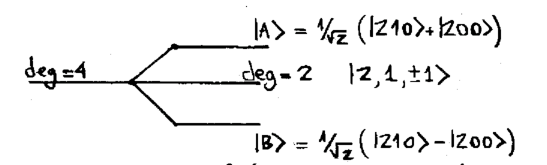
\includegraphics[width=0.6\textwidth]{images/teo2_20.pdf}
	\end{center}
	\caption{}
\end{figure} 

\subsection{Corrimiento de la energía a orden 2 (con degeneración)}

Sea que a orden uno se rompe toda la degeneración 
\[
	(H_0 - E_N^0) \Ket{2_N^j} + (V - E_N^{1 j}) \Ket{1_N^j} - E_N^{2 j} \Ket{0_N^j} = 0
\]
Entonces la corrección a segundo orden de la energía será:
\[
	\Braket{0_N^j | H_0 - E_N^0 | 2_N^j} + \Braket{ 0_N^j | V - E_N^{1 j} | 1_N^j} = E_N^{2 j}
\]
\[
	\Braket{ 0_N^j | V | 1_N^j} = E_N^{2 j}
\]
pues $\Braket{0_N^j|0_N^j}= 0$ pero 
\[
	\Ket{1_N^j} = \sum_{k,i\neq 1} b_k^i \Ket{\varphi_k^i} + \sum_i b_N^i \Ket{\varphi_N^i}
\]
\[
	\Braket{0_N^j|1_N^j} = 0 = \sum_{k,i\neq 1} b_k^i \braket{0_N^j|0_K^i} + 
		\sum_i b_N^i \braket{0_N^j|0_N^i}
\]
falta desarrollo ... [info en mis originaales]

\[
	E_N^{2j} = \sum_{p\neq N} \frac{|\Braket{0_N^j|V|0_p^i}|^2}{E_N^0 - E_p^0}
\]
donde $N$ es un estado degenerado y la suma es entre los $i$ posibles.

\section{Estructura fina del átomo de hidrógeno}

La solución tradicional del átomo de H usa el potencial coulombiano. Esto desemboca en las funciones 
$\Ket{n,\ell,m}$, sin embargo la introducción de ajuste como {\it perturbaciones} rompe algo la degeneración.
\[
	H_0=\frac{p^2}{2m} - \frac{e^2}{r} \qquad E_n = -\frac{\alpha^2m_e^2c^2}{2n^2} \qquad 
	a_0 = \hbar^2/(m_ec^2)
\]
\[
	v/c = p/(mc) = \alpha = \frac{e^2}{\hbar c} \approx 1/137
\]
donde $a_0$ es el radio de Bohr, $\alpha$ es la constante de estructura fina .
Tenemos 
a) Corrección cinemática (relativista)
\[	
	E = c \sqrt{p^2 + m_e^2c^2} = m_ec^2\sqrt{1 + p^2/(m_e^2c^2)} \approx 
	m_ec^2 \left( 1 + \frac{1}{2}\frac{p^2}{m_e^2c^2} + \frac{3}{8}\frac{p^4}{m_e^4c^4} \right)
\]
\[
	E \approx m_ec^2 + \frac{p^2}{2m_e} + \frac{3p^4}{8m_e^3c^2}
\]
y esta corrección va como $W_{mv}/H_0 \sim \alpha^2$.

b) Acoplamiento spín-órbita
Se puede pensar considerando un $e^-$ en reposo con un protón orbitando que genera un $\vb{B}_{eff}$
\[
	W_{so} = \frac{e^2}{2m_e^2c^2} \frac{\vb{L}\cdot\vb{S}}{R^3} = -\vb{\mu}\cdot\vb{B}_{eff}
\]
y la corrección va como $W_{mv}/H_0 \approx \alpha^2$.

c) Término de Darwin o de contacto
\[
	W_D = \frac{\hbar^2}{8m_e^2c^2} \nabla^2 V(r)
\]
que va como  $W_{D}/H_0 \approx \alpha^2$.

Hay otras correcciones hiperfinas que provienen del spín del electrón y del spín del protón. Pero van como 
$\alpha^2/2000$.
Si consideramos el sistema con 
\[
	n=2 \; \ell=0,1 \quad m_\ell = 1,0,-1 \quad m_s=1/2,-1/2
\]
serán ocho estados $\Braket{n,\ell,m_\ell,m_s}$ (base completa).
\[
	W = \underbrace{W_{mv}}_{\sim p^4} + \underbrace{W_{so}}_{\sim \vb{L}\cdot\vb{S}} + 
	\underbrace{W_D}_{\sim |\vb{r}|}
\]
y W es par ante $\Pi$ y sólo habrá elementos de matriz $\neq 0$ que sean de la misma paridad.
\[
	\begin{matrix}
	2s & \qquad 2p \\	 
	\end{matrix}
\]
\[
\begin{matrix}
 2s\\
 2p\\
\end{matrix}
	\begin{pmatrix}
	[2\times 2] & \\
	& [ 6\times 6 ] 
	\end{pmatrix}
\]
$\Ket{2s}$ es par ($\ell=0$) y $\Ket{2p}$ es impar ($\ell=1$) y entonces $\Ket{2s}, \Ket{2p}$
no están conectados.

De manera que hay ocho estados $\Ket{n=2,\ell,m_\ell,s,m_s}$ que al calcular esta perturbación $W$
resultan 
\begin{figure}[htb]
	\begin{center}
	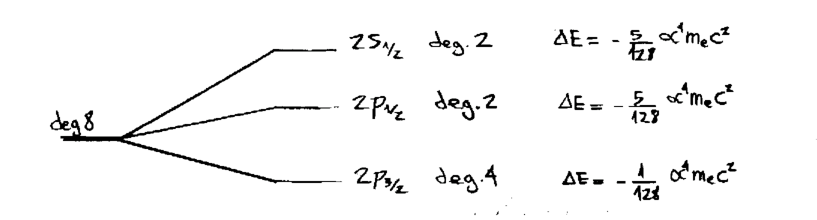
\includegraphics[width=0.9\textwidth]{images/teo2_21.pdf}
	\end{center}
	\caption{}
\end{figure} 

El cálculo para las correcciones hiperfinas no condice la experiencia. Se necesita aquí mecánica cuántica 
relativista. Los dos primeros niveles tienen la misma $\Delta E$ porque en MCR se ve que 
\[
	E = E(n,j) 
\]
es decir que no depende directamente de $\ell,s$.

Un sketch de los métodos perturbativos
\[
	H_0 = \begin{pmatrix}
	       E_1 & \\
	       & E_2 & \\
	       & & E \\
	       & & & E\\
	       & & & & ...\\
	       & & & & & E\\
	       & & & & & & E_3\\
	       & & & & & & & E_4
	      \end{pmatrix}
	      \hspace*{10mm}
	      V =
		\begin{pmatrix}
		& \\
		& \\
		& & V_3 \\
		& & & V_4 \\
		& & & & ... \\
		& & & & & V_{nn} \\
		& \\
		& 
		\end{pmatrix}
\]

En $H$ tenenmos un bloque de energías degeneradas y se diagonalizará el bloque 
correspondiente en la matriz del potencial perturbativo $V$.




% \bibliographystyle{CBFT-apa-good}	% (uses file "apa-good.bst")
% \bibliography{CBFT.Referencias} % La base de datos bibliográfica

\end{document}
